\chapter{Semantic Mapping}\label{chap:semantic-mapping}

% motivation
Humans associate concepts to areas that relate to the functionality of those. That
association is either useful by explaining where to find certain objects as well to
understand the types of activities to perform on it. In a 

Those human-concepts are meant to be meaningful for humans and by incorporating conceptual
knowledge about them it is expected to improve the agent 
% semantic mapping definition
In this context semantic mapping is seen as the process of building a representation of
the environment which associates spatial entities with a set of defined spatial concepts (i.e.\ human concepts).

% importance of conceptual knowledge
% application of conceptual knowledge
It is expected that by being able to reason over those semantics an agent can better
understand human environments and increase its efficiency when performing human-tasks on them.
By handling this conceptual knowledge the agent becomes aware of 


% challenges and need for representing uncertainty
The goal of a spatial representation is to provide the agent with a view about the environment
that allows it to reason beyond its sensory horizon.

 Such a representation is by its nature
imperfect, incomplete, inaccurate and invalid.

world that allows the agent to perform reasoning over it and efficiently perform tasks.
It should also give the agent ability to reason about parts 
Such a representation cannot be perfect since the methods and information are uncertain

% here a here a method is used that does semantic mappping and representes conceptual knowledge
% on a probabilistic fashion.



It is therefore clear that the need to handle information on an high-level semantic and
probabilistic fashion arises not only for efficiency reasons but also from the desire
of being able to communicate and reason on those aspects.
In order to fully explore the semantic properties and their relations it is necessary to
detect and classify semantic aspects as well to understand the relationships between them.
That conceptual knowledge is important and any limitations on it will limit the capacities
of an agent to reason. 

This thesis motivation lies on developing methods for detecting knowledge gaps
on the semantic knowledge of a mobile agent. For that the semantic mapping system
implemented on \gls{Dora} proposed by \cite{pronobis2011phd} was used as a base.


\section{Architecture Overview}
Pronobis~\cite{pronobis2011phd} presents a system architecture working in indoor environments using
non\hyp{}omnidirectional laser and visual sensors for semantic mapping. The system integrates cues such as geometry,
object presence and appearances and is able to perform inference across any semantic properties,
for example for the purpose of place categorization.
The introduced system is built around a spatial knowledge representation~\cite{pronobis2010ias} and it has not only been tested on real-scenarios
and performance tested across several conditions~\cite{pronobis2007iros} but also shown
to be tailored to effectively solve tasks arising on mobile robotics~\cite{hanheide2011ijcai}.

Besides that the spatial knowledge representation has been drawn with an high-focus on probabilistic
and uncertain reasoning, human interaction and life-long learning capabilities.
For that it was considered an excellent base defining not only the concepts and
requirements of an high-level semantic representation but also the information flow
between all the layers involved on the agent.

Being able to perform probabilistic inference on all available information Such a representation is suitable to detect novel concepts.


The system is implemented on \Gls{Dora} and a brief overview of its architecture is
given in the following sections.

\section{Spatial Knowledge Representation}
\cite{pronobis2010ias} proposes a spatial knowledge representation sub-divided into four layers.
Each layer focus on different aspects of the world, abstractions levels of the spatial knowledge
and different spatial scales. Each uses different spatial entities and relate to the agent
goals in different ways:

In the lowest abstraction level the sensory layer represents the most immediate and short term
accurate representation of the world. Above, the place layer discretizes the continuous
space into. The categorical layer focus on knowledge of low\hyp{}level, long\hyp{}term
categorical models of the sensory information. And at the higher level the conceptual map
associates concepts to areas such as rooms (see \autoref{fig:spatial-knowledge}).

\begin{figure}[h]
\centering
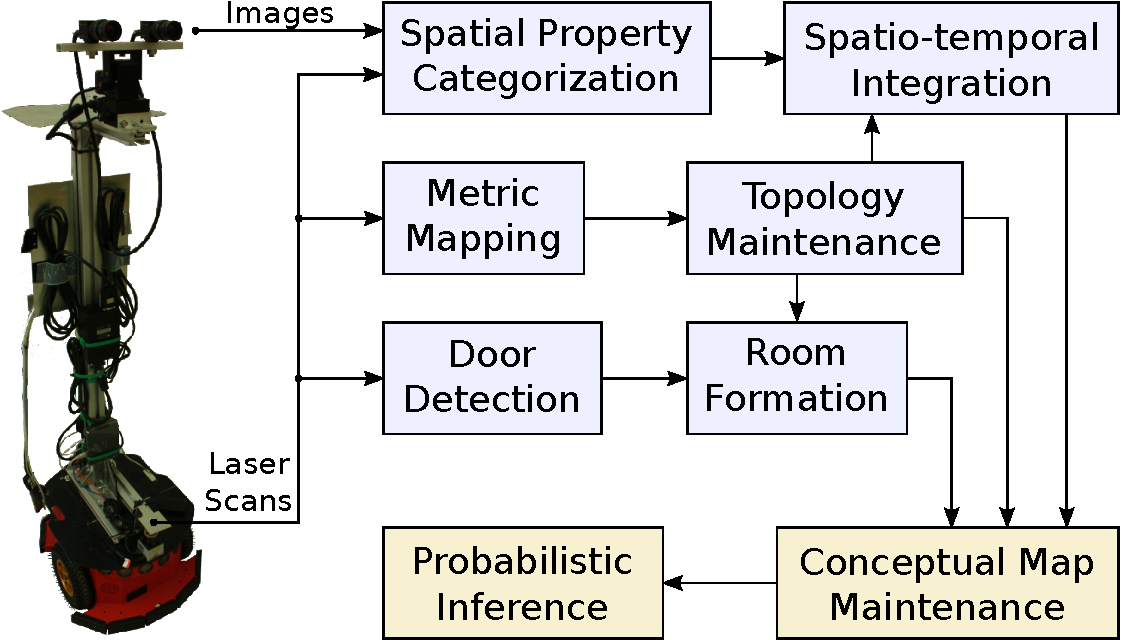
\includegraphics[width=0.7\textwidth]{figures/dora-architecture.pdf}
\caption{\label{fig:spatial-knowledge}Layered structure of the spatial representation.
         The conceptual layer illustrates part of the ontology representing both instance
         and pre-defined world knowledge.}
\end{figure}

\subsubsection*{Sensory Layer}
The sensory layer keeps a detailed representation of the immediate surrounds of the agent.
That representation is based on directly sensed inputs as well on data-fusion for short
time\hyp{}intervals.

It is responsible for providing the agent with an exact position and to accurately position
low\hyp{}features and landmarks. The information is stored with associated uncertainty it
is highly susceptible to be replaced with newer versions. Also old or distant information
is forgotten.
By tracking the surrounds for short amount of times it provides an accurate representation
that can be used to locate and guide the agent on low\hyp{}level movements.

\subsubsection*{Place Layer}
The place layer is responsible for maintaining a bottom\hyp{}up discretization of the
continuous space. On it the world is represented as a collection of discrete spatial
entities, called places, together with connectivity information.

Each place is defined with the features from the sensory layer and with spatial relations
to other places. Connectivity here, stands for ability to travel directly between the
places. Additionally places can be created for areas not yet explored allowing to introduce
virtual place holders to places that would eventually be uncover if the agent moved there.

The places are also considered stable on long\hyp{}term and can be used to help the agent
performing localization and planning longer distance motion planning. This higher level
representation although uncertain allows to model connectivity and relaxed spatial relations.

\subsubsection*{Categorical Layer}
The categorical layer holds the generic long-term, low-level representations of categorical models
of the agent's sensory information.
The knowledge represented by this layer is not instance specific. It is the knowledge
required to determine certain features indicate the presence of an entity of certain
category. E.g.\ the knowledge required to detect objects, landmarks or describe room appearances.
Other properties may as well be defined for example shape, color, edges and size properties
are all defined in terms of low\hyp{}level features.

This layer is responsible for representing knowledge on how to extract properties used
by the conceptual layer.
Although not mandatory, in many cases the categories represented by it will map to human concepts
and not to the internal concepts of the agent.
The type of properties handled by this layer may require incredible complex models and for
that they might be trained on a supervised fashion.

\subsubsection*{Conceptual Layer}
The conceptual layer provides an ontology that represents a taxonomy of the spatial concepts
and their relations with the properties represented on the categorical layer.
This associates semantic meaning to those properties that is useful for human-agent iteration
and provides relations that can be verbalized and explained with the ontology.

It provides also knowledge between the semantic concepts and their instances of those concepts.
Including definitions of spatial concepts related to space segmentation as well to semantic
categorization of those spatial entities.
E.g.\ rooms are commonly split by doors, rooms exist in a floor, a building has floors, milk is
likely to be found on kitchens, etc\dots

By providing information for segmentation, semantic mapping to concepts and relations between those
concepts, the knowledge represented on this layer allows the agent to explain and reason close to
the human concepts. The knowledge represented here is considered to be valid through very long
periods of time or even life\hyp{}long.


\section{System Structure}
The \Gls{Dora} system~\cite{hanheide2011ijcai} consists of several co-operating
sub-systems, all of which actively use or maintain the spatial knowledge representation
(see \autoref{fig:dora-architecture}).


\subsection{Features}
\label{sec:dora-features}
The \emph{categorical layer} requires classifiers with the ability to categorize 

\section{Conceptual Map}
\label{sec:conceptual-map}
As \gls{Dora} moves through the environment it builds a \emph{conceptual map}: a structural and
probabilistic representation of the space instantiated as a \emph{graphical model}.
It includes taxonomy of human\hyp{}compatible spatial concepts which are linked to the sensed 
instances of these concepts drawn from lower layers. It is the conceptual layer which 
contains the information that kitchens commonly contain cereal boxes and have certain 
general appearance and allows the robot to infer that the cornflakes box in front of the 
robot makes it more likely that the current room is a kitchen. The conceptual layer is 
described in terms of a probabilistic ontology defining spatial concepts and linking 
those concepts to instances of spatial entities (see the example of the ontology in
\autoref{fig:dora-architecture}).

Based on this design, a \emph{chain graph} model is proposed as a 
representation for performing inferences on the knowledge represented in the conceptual 
layer. Chain graphs are probabilistic graphical models that combine the properties of 
both Bayesian Networks and Random Markov Fields. This results in an efficient approach to 
probabilistic modeling and reasoning about conceptual knowledge.

\begin{figure}[h]
\centering
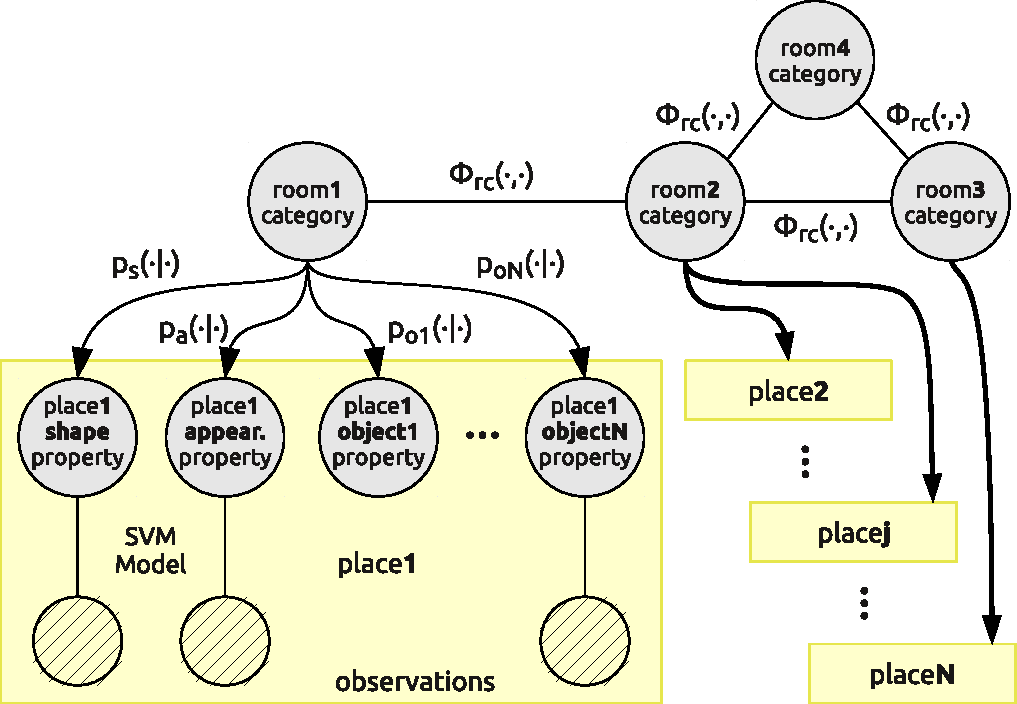
\includegraphics[width=0.75\textwidth]{figures/chaingraph.pdf}
\caption{\label{fig:chain-graph}Example chain-graph instantiated from the \emph{conceptual layer}.}
\end{figure}

%The conceptual layer structures the sensed environment together with the conceptual knowledge
%in order to create a structured probabilistic representation of the world.
An exemplary chain graph corresponding to the conceptual map ontology is presented
in \autoref{fig:chain-graph}. 
Each discrete place identified in the environment is represented by a set of random variables, 
one for each class of relation linked to that place. These are each connected to a random variable
over the categories of rooms, representing the ``is-a'' relation between rooms and their categories. 
Moreover, the room category variables are connected by undirected links to one another according 
to the topological map. The remaining variables represent: shape and appearance properties of space 
as observed from each place, and the presence of objects. 
These are connected to observations of features extracted directly from 
the sensory input. Finally, the 
distributions $p_{s}(\cdot|\cdot)$, $p_a(\cdot|\cdot)$, $p_{o_i}(\cdot|\cdot)$ 
represent the common sense knowledge about shape, appearance, and object co-occurrence, respectively. 
They allow for inference about other properties and room categories e.g. that the room is likely to be a kitchen,
because you are likely to have observed cornflakes in it. 

The use of graphical models to describe distributions of variables has useful properties.
First, they permit inference about uncertain conceptual knowledge. At the same time, they are 
generative models and therefore allow to calculate the probability
on any given subset of variables of the graph, allowing the system to work even when some
information is missing.

\subsection{Factor Graphs}
Although the conceptual layer works with \emph{chain graphs}~\cite{lauritzen2002chain},
those can be converted into \emph{factor graphs}~\cite{kschischang2001factor}.
Factor graphs have been introduced in \autoref{sec:graphical-models} and are used
throughout this thesis as they provide an easier manipulation due to factorization.

Moreover, there exist efficient implementations of inference engines operating on factor
graph representations~\cite{Mooij_libDAI_10}.
Describing the distribution function in terms of graphs permits the use of those engines to
efficently calculate marginals on any given subset of variables by exploiting conditional
independence between variables.

\subsection{Uncertain Sensing and Implicit Factors}
\label{sec:cues-from-low-level}
In a realistic scenario, classification tasks are by their nature uncertain.
And although a trained classifier is able to decide which class is more likely, there is
interest in handling uncertainty produced by those to make decisions more robust.

By modelling the classifiers as an implicit function $\phi_{classifier}(c, x)$ it becomes
possible to model the uncertainty of the decision given the presence of the sensed low-level
features $x$. The presence of those implicit models no longer allow calculation of the
normalization factor over the whole graph as there is no explicit model for either the
low\hyp{}level features $X$ (e.g.\ $X$ can be an image received from a visual sensor)
or for $\phi_{classifier}$ (e.g.\ the classifier can be an \gls{SVM}).

Nonetheless it is still possible to calculate any probability given that the features $X$
are observed. For that instead of modelling the variables $X$ and explicitly describing
the factor $\phi_{classifier}$ it is enough to replace it by an observed factor
$\phi_{classifier}(c|x)$ as shown on \autoref{fig:implicit-factor}.


\begin{figure}[h]
\centering
\subfloat[]{
\begin{tikzpicture}
  \node [matrix,matrix anchor=mid, column sep=20pt, row sep=10pt,ampersand replacement=\&] {
    \& \& \node (graph) [] {\dots}; \& \& \\
    \& \& \node (prop) [latent] {$c$}; \& \& \\
    \& \& \node (fac) [factor] {}; \& \& \\
    \& \& \& \& \\
    \node (x1) [obs] {$x_1$}; \&
    \node (x2) [obs] {$x_2$}; \&
    \node (x3) [obs] {$x_3$}; \&
    \node (xi) [] {\dots}; \&
    \node (xn) [obs] {$x_n$}; \\
  };
  \draw [-] (prop) -- (graph);
  \draw [-] (prop) -- (fac);
  \draw [-] (fac) -- (x1);
  \draw [-] (fac) -- (x2);
  \draw [-] (fac) -- (x3);
  \draw [-] (fac) -- (xi);
  \draw [-] (fac) -- (xn);

  \node (captfactor) [right=2pt of fac] {\footnotesize{$\phi_{classifier}(c, x)$}};
\end{tikzpicture}
}
\qquad
\subfloat[]{
\begin{tikzpicture}
  \node [matrix,matrix anchor=mid, column sep=20pt, row sep=10pt,ampersand replacement=\&] {
    \& \& \node (graph) [] {\dots}; \& \& \\
    \& \& \node (prop) [latent] {$c$}; \& \& \\
    \& \& \node (fac) [factor] {}; \& \& \\
    \& \& \node (hidden) [latent,draw=none] {}; \& \& \\
  };
  \draw [-] (prop) -- (graph);
  \draw [-] (prop) -- (fac);
  \node (captfactor) [right=2pt of fac] {\footnotesize{$\phi_{classifier}(c | x)$}};
\end{tikzpicture}

}

\caption{\label{fig:implicit-factor}By modelling classifiers as implicit factors it is
possible to perform inference on the graphical models handling the uncertainty measures
produced by those classifiers.}
\end{figure}

